\section{Organisatorische Änderungen}

\subsection{Übersicht über die Repositories}
Das ursprüngliche Projekt bestand aus zwei Teilen: der Android App, als lokaler Client, und einem Backend, dessen Service den Bot beinhaltet. Diese Teile waren bisher zusammen in einem einzigen Repository. Das Zusammenlegen hatte eine gewisse Unübersichtlichkeit zur Folge. Daher haben wir für jedes Teilprojekt ein eigenes Repository angelegt. Die Aufteilung zwischen App und Backend wurde beibehalten, lediglich kam noch ein zusätzlicher Teil hinzu, die Service-API-Library. Damit ist die aktuelle Aufteilung auf Github wie folgt:
\begin{itemize}\itemsep0pt
	\item Altes Repository unserer Vorgänger - https://github.com/TeamChatbot/chatbot
	\item Aktuelle Android App - https://github.com/TeamChatbot/Hablame-Android-App
	\item Aktuelle Service-API-Library - https://github.com/TeamChatbot/hablame-service-api
	\item Aktuelles Service-Botbackend - \\https://github.com/TeamChatbot/Hablame-BotBackend
\end{itemize}
Durch diese Aufteilung kann besser und unabhängiger an den einzelnen Teilprojekten gearbeitet werden.

\subsection{Dokumentation im Allgemeinen}
Für die Dokumentation gibt es nun mehrere Anlaufstellen. In Redmine gibt es ein integriertes Wiki welches wir bereits mit einigen Informationen zu allgemeine Dingen wie Logindaten und den einzelnen Repositories, aber auch zu genutzten Technologien wie beispielsweise das Git-System gefüllt.\footnote{Projekt Wiki in Redmine: http://194.95.221.229/redmine/projects/hablame/wiki/}
Zusätzlich zu dem Wiki gibt es in jedem Repository ein Readme, das nochmal zusätzlich einen Überblick über das dortige Projekt gibt.\\
Die Dokumentation des Programmcodes ist mittels dem Java Tool JavaDocs umgesetzt worden. Die damit generierten Dokumentationsseiten sind im jeweiligen Repository auf Github zu finden.

\subsection{Die Service-API-Library}
Um die Nutzung des Backends zu vereinfachen wurde ein weiteres Teilprojekt erstellt: die Service-API-Library. Dieses Projekt bietet einen einfach zu handhabenden Client zur Nutzung des Bot-Services. Dafür bietet dieser Methoden zur jeder Schnittstelle des Backends.\\
Durch dieses Vorgehen ergibt sich der Vorteil, dass somit eine einheitliche, leicht zu nutzende Schnittstelle für Nutzerprogramme geboten wird, welche auch in weiteren Anwendungen integriert werden kann (z.B. in eine Desktopanwendung).\\
Als Basis für die Rest-Kommunikation wird die Bibliothek UniREST von Mashape.\footnote{Unirest: http://unirest.io/}

\subsection{Aktuelle Aufgabenverteilung der Teilprojekte}
Durch das Hinzufügen der Service-API-Library ergibt sich nachfolgend dargestellter Gesamtaufbau:

\begin{figure}[h]
\centering
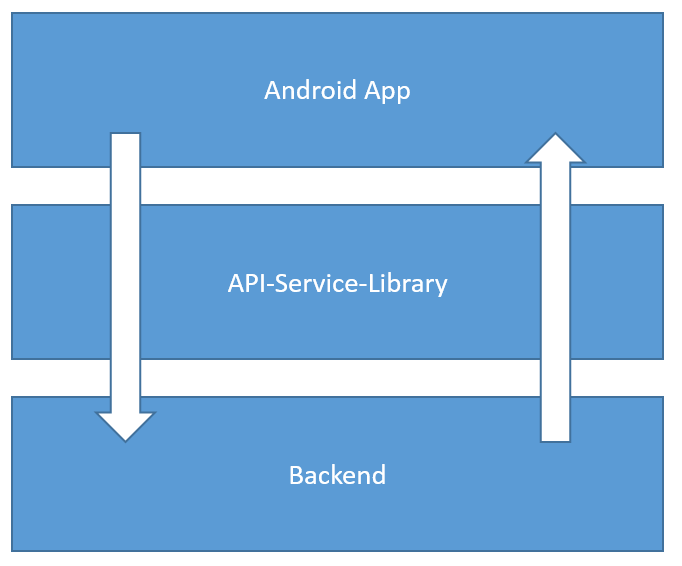
\includegraphics[width=0.7\linewidth]{ks/graphics/arch.png}
\caption{Gesamtaufbau Hablame}
\label{fig:arch}
\end{figure}

Jedes Teilprojekt behandelt ein Teilproblem des Gesamtsystems.
Android App:
\begin{itemize}\itemsep0pt
	\item Umwandlung gesprochener Sprache in Text ("Speech-To-Text")
	\item Umwandlung von Text in gesprochene Sprache ("Text-To-Speech")
	\item Weiterleiten der Informationen mittels der API-Service-Library an das Backend
\end{itemize}
API-Service-Library:
\begin{itemize}
	\item Erstellen der Anfragen an das Backend
	\item Weitergabe der Backend-Antworten an das aufrufende System
\end{itemize}
Backend:
\begin{itemize}
	\item Hosting und Konfiguration des Chatbots
	\item Auswerten der Serviceanfragen
\end{itemize}
